\section{System architecture}

The system consists mainly of three parts, of which one is used for generating test data and two are used for the actual reinforcement learning.
On the one hand, there exits a Python-based program that can be used to generate synthetic training images with text on them.\footnote{The program's source code can be found on GitHub.\cite{GitHubDatasetGenerator}}. 
This program is called the \textit{dataset-generator}.
On the other hand, there exist two programs also based on Python which provide both the environment and the agent used for the reinforcement learning's training and testing.\footnote{The source code of those programs can be found on GitHub as well.\cite{GitHubTextLocalizationEnvironment}\cite{GitHubTextLocalizationAgent}}. 
Those programs are called \textit{text-localization-environment} and \textit{text-localization-agent} respectively. 

Both the \textit{dataset-generator} and the \textit{text-localization-agent} program use the Python package \textit{click}\cite{PythonPackageClick} for offering command-line interfaces that allow users to change the programs' parameters without having to change their source code.
This is especially useful when running the programs on computers accessed via a remote connection (e.\,g. via SSH), as it often is the case when working on machine learning projects.

A typical use-case for using the system is to (a) generate synthetic training data using the \textit{dataset-generator}, (b) installing the \textit{text-localization-environment} for later usage by the agent and (c) training and/or evaluating one or multiple agents using the \textit{text-localization-agent}. 
In the following paragraphs, the three programs and their usage options are described more in-depth.

\subsection{The dataset-generator program}

As briefly introduced before, the \textit{dataset-generator} is a program that can be used for generating synthetic training data for usage in machine learning projects related to the bounding box detection (localization) of text on images. 
It does so by using the Python package Pillow\cite{PythonPackagePillow} to load one or multiple fonts, create images of a specific size and render one or multiple words of text onto those images.
The words themselves come from a public domain word list originally contained in the original BSD project project.\cite{BSDWordlist}

For the generation of image datasets, users can control the images' width, their height, the amount of images to generate, the location of a word list (in a format similar to the word list contained by default, as described above), a seed used for the random calculations within the program as well as whether the program should use a debug mode (in which it renders AABB outlines around the corresponding words).

Figure \ref{fig:dataset-generator-sample-output} shows two sample images created by the \textit{dataset-generator}, one using the default settings and one explicitly having the \textit{debug} flag set to true. 
In addition to the images, the program also creates a \texttt{.npy} file containing the AABB locations of the words in the images in a Numpy-encoded way as well as a \texttt{.txt} file containing the relative locations of the generated images.

\begin{figure}[h!]
    \begin{subfigure}[t]{0.5\textwidth}
        \centering
        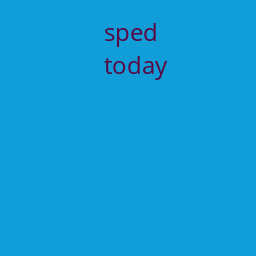
\includegraphics[width=0.8\textwidth]{figures/dataset-generator-sample-1.png}
        \subcaption{Debug mode disabled (default setting)}
    \end{subfigure}
    \begin{subfigure}[t]{0.5\textwidth}
        \centering
        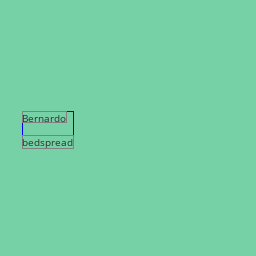
\includegraphics[width=0.8\textwidth]{figures/dataset-generator-sample-debug.png}
        \subcaption{Debug mode enabled. The blue and gray boxes indicate the AABB of the single words and of the whole “text” block}
    \end{subfigure}
    \caption{Two sample images created by the \textit{dataset-generator}}
    \label{fig:dataset-generator-sample-output}
\end{figure}

\noindent Together with the \texttt{.npy} and the \texttt{.txt} files, the images can be used by the \textit{text-localization-environment} program as described in the following section.

\subsection{The text-localization-environment program}

The \textit{text-localization-environment} program is designed to conform to OpenAI Gym's environment interface \textit{Env}\cite{OpenAIGym} by implementing the three following methods:
\begin{quote}
    \begin{itemize}
        \item reset(self): Reset the environment's state. Returns observation.
        \item step(self, action): Step the environment by one timestep. Returns observation, reward, done, info.
        \item render(self, mode='human', close=False): Render one frame of the environment. The default mode will do something human friendly, such as pop up a window. Passing the close flag signals the renderer to close any such windows.
    \end{itemize}\cite{OpenAIGymReadme}
\end{quote}
In general, the environment is based on the algorithm described in the paper\cite{caicedo2015active} which we based our research on:
The environment offers a total of 9 actions to the agent (and thus uses a \textit{discrete} action space).
Those actions are exactly the same as the one used in the paper mentioned above, and are visualized in figure \ref{fig:environment-actions-from-base-paper}.

\begin{figure}[h!]
    \centering
    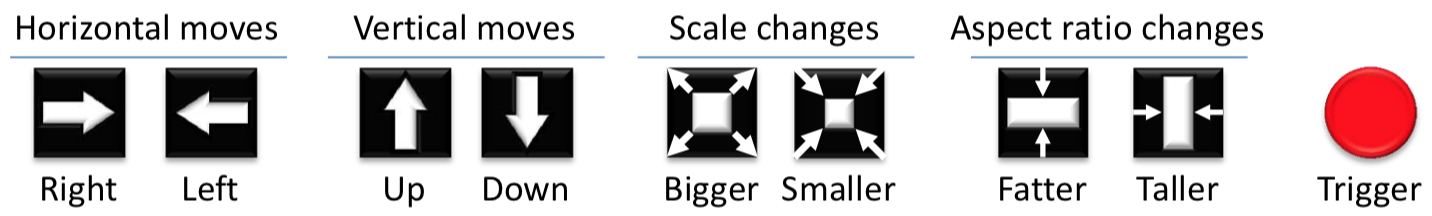
\includegraphics[width=0.7\textwidth]{figures/environment-actions-from-base-paper.png}
    \caption{The actions offered by the environment to the agent\cite{caicedo2015active}}
    \label{fig:environment-actions-from-base-paper}
\end{figure}

After being initialized with a set of images (indicated by a corresponding \texttt{.txt} file, as described above) and the ground truth bounding boxes (contained in a \texttt{.npy} file), the environment acts as a kind of state machine which can be controlled by the three main methods described above. 
For calculating the observation in the \textit{reset} and \textit{step} methods, the environment uses a feature extractor – in our case, we used VGG16\cite{VGG16} in the beginning and replaced it with ResNet\cite{ResNet} later.
In order to control whether this feature extractor runs on the GPU, the environment can be initialized with a corresponding parameter indicating the ID of the GPU to be used.

For calculating the reward returned by the \textit{step} method, the environment calculates the best intersection over union (IoU) of the current bounding box and any of the ground truth bounding boxes. 
Depending on whether this IoU changed positively or negatively in respect to the one calculated in the step before, the reward is either $+1$ or $-1$. 
During the course of the project, we also introduced two more means for increasing the likelihood of the agent using the \textit{trigger} action: We (a) made the environment count the amount of consecutive steps taken that did not change the IoU in any way (and give a negative reward of $-1$ whenever this count exceeds 3 steps) and (b) introduced a duration penalty (with a default value of $0.03$) which is multiplied by the amount of steps taken since the last time the \textit{reset} method was called and subtracted from the reward.

Although the \textit{text-localization-environment} program is theoretically independent from the agent using it (as proposed in the OpenAI specification), it usually is used together with such an agent.

The program allowing the trainign and testing of such agents is described in the following section.
